\documentclass[tikz]{standalone}

\colorlet{FilledSurface}{blue!20}
\colorlet{FilledSurfaceGroupOne}{blue!20}
\colorlet{FilledSurfaceGroupTwo}{red!20}
\colorlet{FilledSurfaceGroupThree}{green!20}
\colorlet{FilledSurfaceGroupFour}{magenta!20}
\colorlet{FormulaBackground}{green!10}
\colorlet{FormulaFrame}{green}


\usetikzlibrary{calc, intersections, angles}

\begin{document}
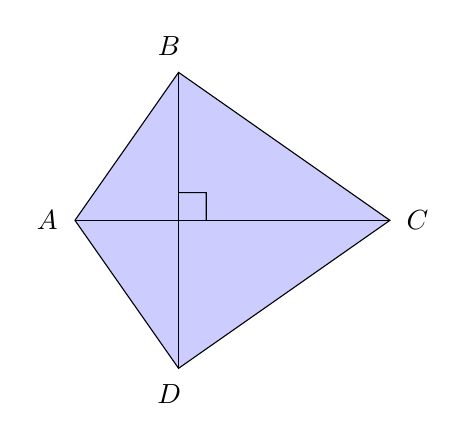
\begin{tikzpicture}

    \def\offset{10pt}
    \def\circumradius{2cm}
    \def\angleA{180}
    \def\angleB{110}
    \def\angleC{0}
    \def\angleD{250}

    \coordinate (center) at (0,0) circle (\circumradius);
    \draw[draw=none, overlay] (0,0) circle (\circumradius);
    \coordinate (A) at ({\circumradius*cos(\angleA)}, {\circumradius*sin(\angleA)});
    \coordinate (B) at ({\circumradius*cos(\angleB)}, {\circumradius*sin(\angleB)});
    \coordinate (C) at ({\circumradius*cos(\angleC)}, {\circumradius*sin(\angleC)});
    \coordinate (D) at ({\circumradius*cos(\angleD)}, {\circumradius*sin(\angleD)});

    \draw[fill = FilledSurfaceGroupOne] (A) -- (B) -- (C) -- (D) -- cycle;

    % Nombrar vértices del cuadrilátero
    \draw ($(center) + (\angleA:\circumradius + \offset)$) node {$A$};
    \draw ($(center) + (\angleB:\circumradius + \offset)$) node {$B$};
    \draw ($(center) + (\angleC:\circumradius + \offset)$) node {$C$};
    \draw ($(center) + (\angleD:\circumradius + \offset)$) node {$D$};

    % Hallar punto de intersección entre las diagonales
    \draw [name path=diagonalAC] (A) -- (C);
    \draw [name path=diagonalBD] (B) -- (D);
    \path [name intersections={of=diagonalAC and diagonalBD, by=I}];

    % Mostrar ángulo entre diagonales
    \path pic [draw, angle radius = 10pt] {right angle = C--I--B};
\end{tikzpicture}
\end{document}
